\section{Planning \& etc.}

Here are the planning notes preceding Brezzvezdna Noč, which show the initial topics considered (in some cases, later abandoned) in preparation for the expedition. These notes are from ICCC's weekend trip to Slovenia in February 2009, typed up on the plane back to London.

\begin{marginfigure}
\checkoddpage \ifoddpage \forcerectofloat \else \forceversofloat \fi
\centering
 \frame{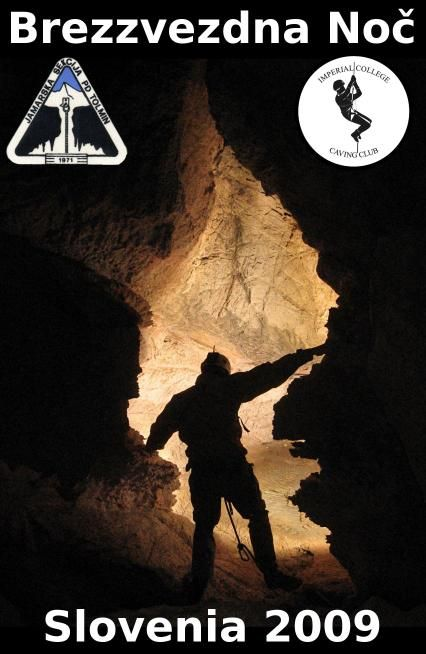
\includegraphics[width=\linewidth]{2009/planning/slov2009_front_logo.jpg}} 
 \caption{The logo for the 2009 expedition. \pen{Jarvist Frost}}
 \label{expologo 2009}
\end{marginfigure}

    \subsection{Move bivi?}
        \begin{itemize}
            \item Imagine will take 	$\approx$ 1 man day effort. Move nearer \passage{Vrtnarija}?
            \item Perhaps just leave till next year (when finally finished with high plateau).
        \end{itemize}
        
    \subsection{Dye Tracing}
        \begin{itemize}
            \item Andrej in contact with water company and government to organise official resurgence tracing, perhaps even possibility of sponsorship / payment.
            \item Permission needed even for very small local traces, due to possibility of detection in Tmin water supply and resulting furore.
        \end{itemize}
        
    \subsection{Slideshow}
        \begin{itemize}
            \item Must be after mid August Slov bank hol
            \item Therefore seems to make sense to have on last weekend of expo
            \item If Sat afternoon, will have to leave promptly to be back at sensible time.
            \item Therefore derig Ravne, pack van and cavers' party on Friday?
        \end{itemize}


\begin{survey}
\centering
\frame{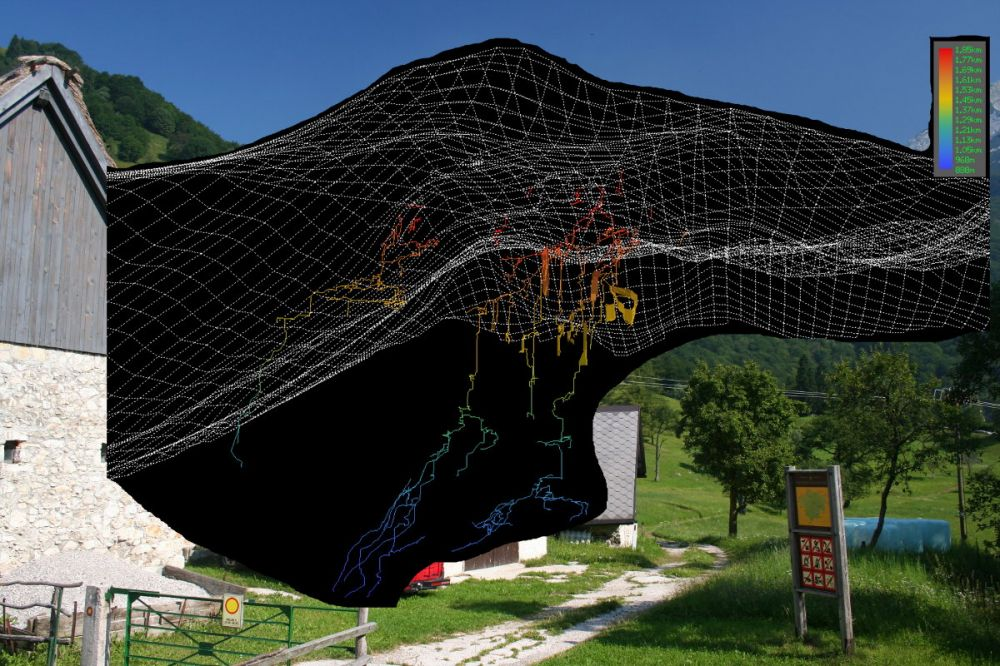
\includegraphics[width=\linewidth]{2009/survey/ravne_survex_100pc_opaque.jpg}}
\caption[Overlay of pre-2009 Survex data with an overground photograph of Tolminski Migovec]{Opaque overlay of Survex data of the cave systems under \passage[mountain]{Tolminksi Migovec} with an overground photograph of \passage[mountain]{Tolminksi Migovec}, taken from \passage[town]{Tolminkse Ravne}.}
\end{survey}


    \subsection{Radio Direction Finding to co locate end of M2 c.f. end of Capt K?}
        \begin{itemize}
            \item Would require placing transitter in \passage{M2}, then pickup equip in \passage{Capt K}\ldots{} bearings from multiple positions to add to survey\ldots{}
        \end{itemize}
\tweet{7:34PM May 20, 2009}{Beast Products is graciously sponsoring us with UG fleeces. Funding from GPF and ICU. Ferry Booked. Slideshow T'min lib 8pm Sat 22nd Aug.}

    \subsection{Underground Camp}
        \begin{itemize}
            \item More fleece snorkels?
            \item Army wool balaclavas?
            \item Chase Beast for products inc. produced version of snorkel?
            \item Fleece liners to go with Nitestar 350x2 (Left,Right Zip), 10mm mats
            \item Mood lighting? Candles? Omni LED?
        \end{itemize}      
        
    \subsection{UG Food}
        \begin{itemize}
            \item Make up freezer-bag meals in UK? Check out Veggie back pack book?
            \item Food dehydrate? Find wholesale dried veggies?
            \item MISO powder!
            \item Go with Tranga, but buy Meths/alcohol before?
        \end{itemize}
        
\recipecorner{Expo Food Ideas}{
    Recipes: http://ramkicooks.blogspot.
    com/ - nice Indian-orientated combinatorial recipe cards. Very good + flexible!\\
        Jarv bought a copy of \textit{Lipsmackin' Vegetarian Backpackin'} which is actually surprisingly good - interesting boiling water + ziplock bag of ingredients super-meals that could be prep'd for UG camp.\\ 
\textbf{UG Food}
    \begin{itemize}
    \item Pita bread + humus work really well
    \item Apples perversely nice 
    \end{itemize}
\mininame{Jarvist Frost}}

    \subsection{Bivi}
        \begin{itemize}
            \item More Tarps
            \item 2nd regulator for Amorph PV panel? Voc too high for current X'tal one. Or just direct connect \& occasionally check for overcharging with multimeter?
            \item Lead-Acid charge spec for various T
            \item Pressure cooker? (McGowan safe?\sidenote{See \textbf{Slop Kaboom} earlier in this book})
            \item Wood oven?
            \item ROCKET STOVE!!! (Tin Snips, Nido tins\ldots{} elbow joint?)
        \end{itemize}
        
    \subsection{High power UG camp stereo?}
        \begin{itemize}
            \item Worth the extra weight, cost ($\approx$ 30 squid) and bother?
            \item Rik + Dan suggest use a car full-range driver, pointless to have Daren box\ldots{}
            \item + 7 day shop SD/MP3 player to use as source
        \end{itemize}
        
    \subsection{Film / audio}
        \begin{itemize}
            \item 10W LED light should be built for UG filming - then just use compact digital camera
            \item Ambient sound recording might be very interesting - maybe even noise-activated recorder?
        \end{itemize}   
        
    \subsection{Survey}
        \begin{itemize}
            \item Survex (CVS) on OLPC lappy
            \item Calibrate compasses (out of London? Kent?) Multi points?
            \item Check + pos make more survey books
        \end{itemize}
\begin{marginfigure}
\checkoddpage \ifoddpage \forcerectofloat \else \forceversofloat \fi
\centering
 \frame{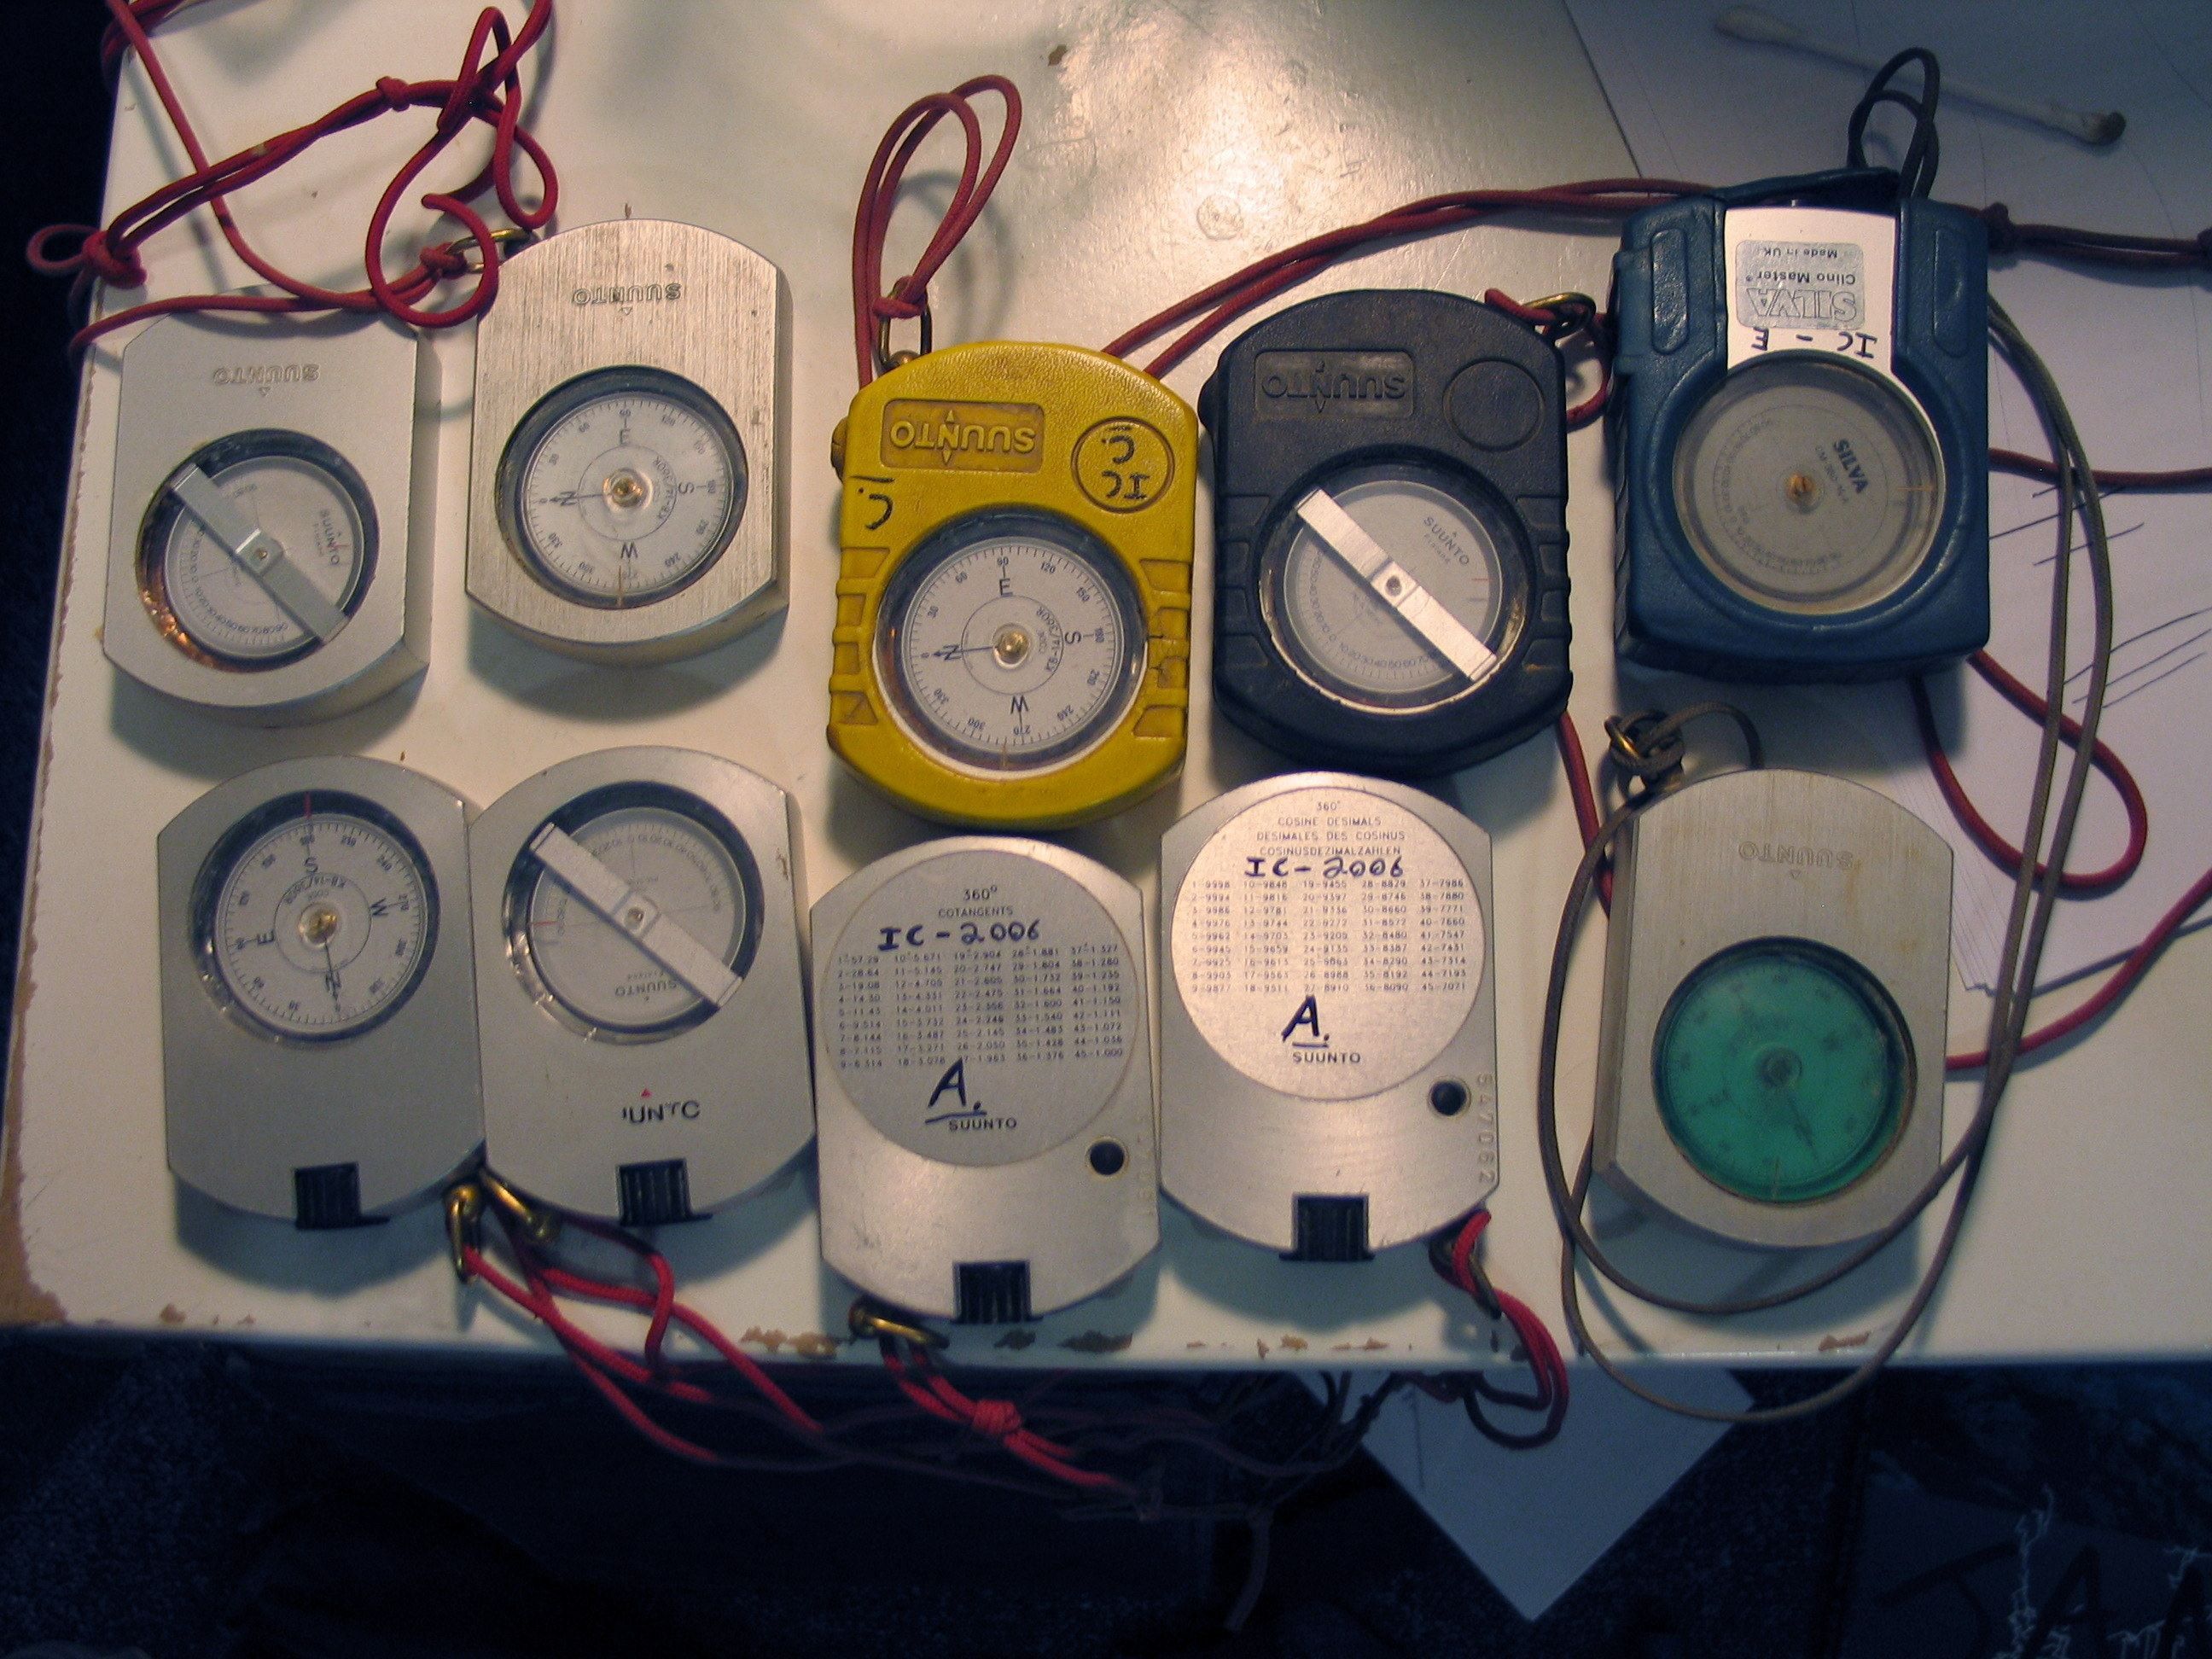
\includegraphics[width=\linewidth]{2009/planning/2009-07-21-02.26.07 - Jarvist Frost - Canon Powershot G5 - Pre-Expo - Instrument Collection--orig.jpg}} 
 \caption{2009's pre-expo collection of survey instruments. \pic{Jarvist Frost}}
 \label{survey collection 2009}
 \end{marginfigure}

\begin{marginfigure}
\checkoddpage \ifoddpage \forcerectofloat \else \forceversofloat \fi
\centering
 \frame{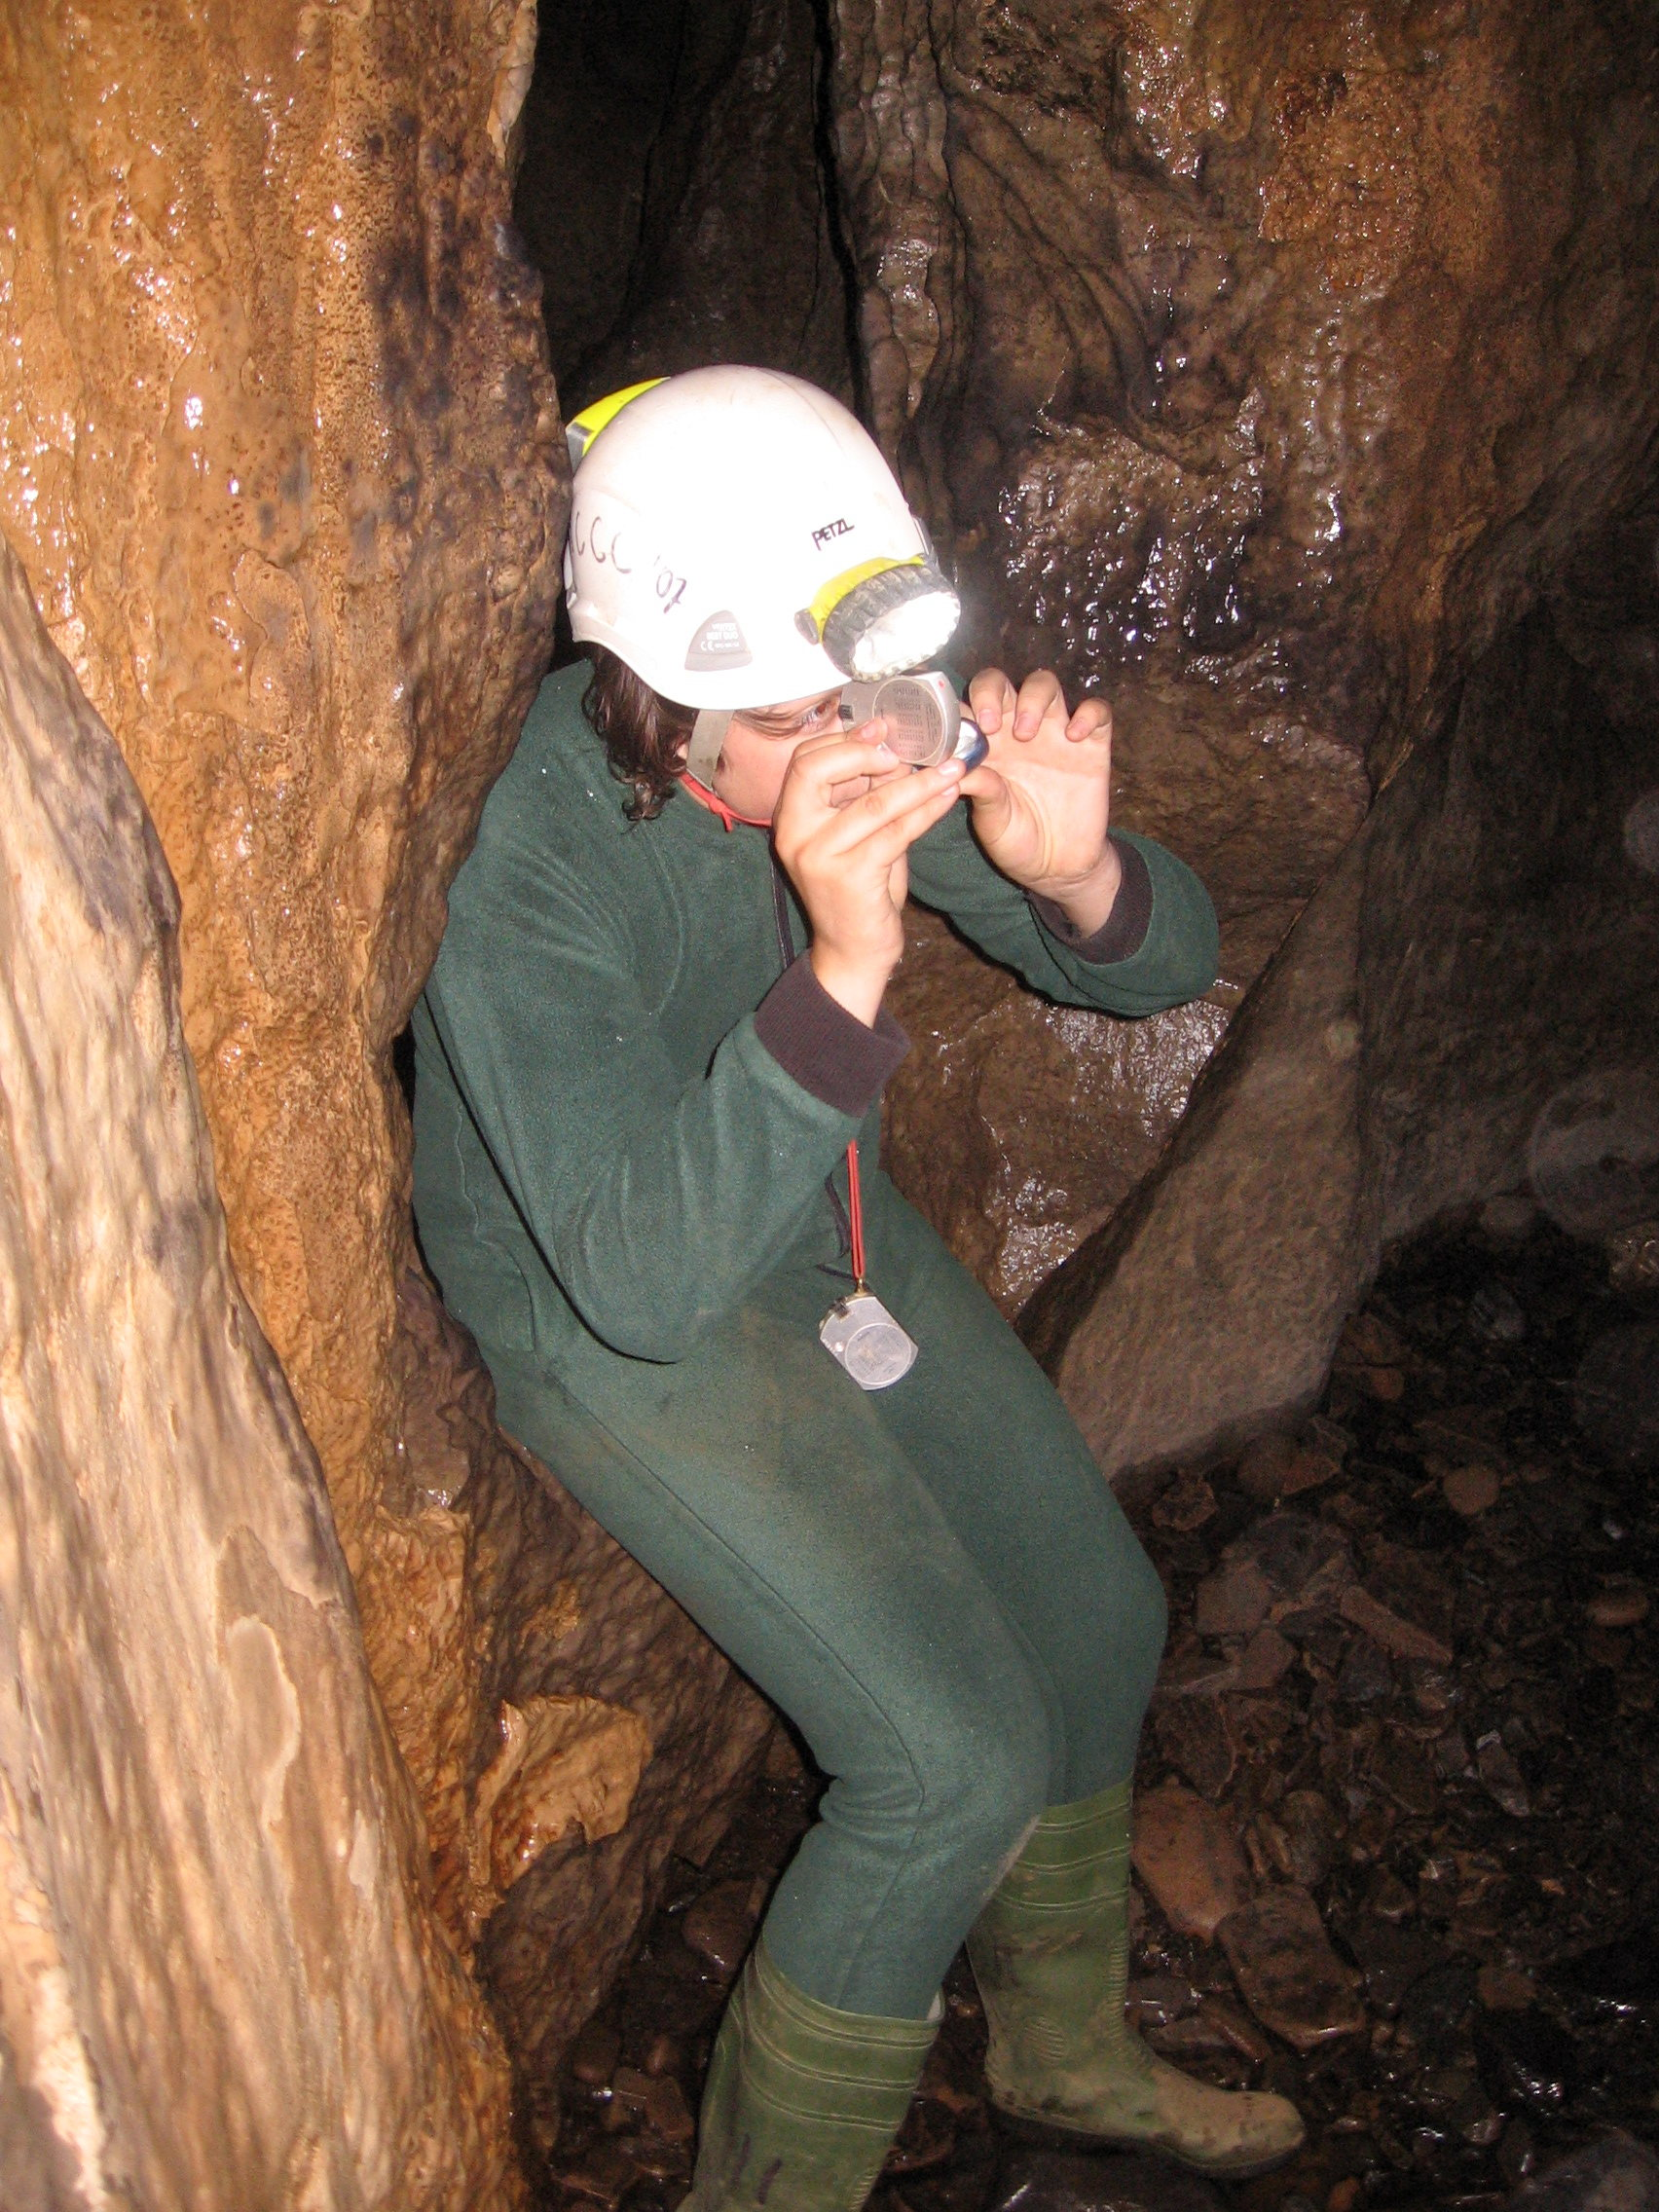
\includegraphics[width=\linewidth]{2009/planning/2009-07-11-16.16.59 - Jarvist Frost - Canon Powershot A520 - Survey practice yordas2--orig.jpg}} 
 \caption{Alex Herriott practicing surveying in \passage{Yordas Cave} prior to the expedition. \pic{Jarvist Frost}}
 \label{survey practice yordas}
\end{marginfigure}  

    \subsection{Surface Survey}
        \begin{itemize}
            \item WAAS measurements of Trig points / tie-in stations - data log to laptop?
            \item Delphi code from nice Italians for transformation to Gauss Kruger - pythonise?
            \item Panorama photo from \passage[mountain]{Kuk}? Calibrated against bearings?
            \item Incorp DEM data more properly - check Survex list for Java program to SVX'afy DEM data (uses landsat info\ldots{}), same as Google earth?
        \end{itemize}
        
    \subsection{Bolts}
        \begin{itemize}
            \item Need lots of Spitz - Lyon?
            \item various sized 8mm stainless throughs for drill bolts
            \item Some more exciting permanent rigging solution? 10mm non-CE throughs? Petzl integrated hangers?
        \end{itemize}
        
    \subsection{First Aid}
        \begin{itemize}
            \item Most injuries are minor burns and flesh wounds from rock - anti sep, burn cream and lots of light dressings used
            \item Serious aid for the serious possiblities (massive petrol burns, broken bones) - TimO\sidenote{Tim studied medicine}
        \end{itemize}
        \name{Jarvist Frost}